% !TeX root = main.tex

\hypertarget{discrete-random-variables}{%
\section{Discrete Random Variables}\label{discrete-random-variables}}

\hypertarget{random-variables}{%
\subsection{Random Variables}\label{random-variables}}

\begin{itemize}
\item
  A \textbf{random variable}, usually written \(X\), is a variable whose
  values are numerical quantities of possible outcomes a random
  experiment.
\item
  A \textbf{discrete random variable} takes on only a finite or
  countable number of distinct values.
\item
  A \textbf{continuous random variable} takes on values which form an
  interval of numbers.
\end{itemize}

\begin{example}

\begin{itemize}
\item
  Rolling a fair dice, the number of dots on the top faces is a discrete
  random variables takes on the possible values: 1, 2, 3, ,4, 5, 6.
\item
  Flipping a fair coin 10 times, the number of heads is a discrete
  random variable takes on the possible values: 1, 2, 3, \ldots, 10.
\end{itemize}

\end{example}

\begin{example}

\begin{itemize}
\item
  The height of an randomly select 10 year-old boy in US is normally
  between 129 cm and 157 cm. So the height is a continuous random
  variable.
\item
  The measure the voltage at an randomly electrical outlet normally is
  between 118 and 122. So the measure of voltage is a continuous random
  variable.
\end{itemize}

\end{example}

\begin{exercise}

Classify each random variable as either discrete or continuous.

\begin{enumerate}
\item
  The number of boys in a randomly selected three-child family.
\item
  The temperature of a cup of coffee served at a restaurant.
\item
  The number of math majors in randomly selected group of 10 students.
\item
  The amount of rain recorded in a small town one day.
\end{enumerate}

\end{exercise}

\hypertarget{probability-distributions}{%
\subsection{Probability Distributions}\label{probability-distributions}}

\begin{itemize}
\item
  The \textbf{probability distribution} of a discrete random variable
  \(X\) is defined by the probability \(P(X=x)\) associated with each
  possible value \(x\) of the variable \(X\). The function
  \(p_X(x)=P(X=x)\) is called the \textbf{probability mass function}.
\item
  A probability distribution of a discrete random variable is usually
  characterized by a table of all possible values \(X\) together with
  probabilities \(P(X)\), or a probability histogram, or a formula.
\item
  A random variable \(X\) (discrete and continuous) always has a
  \textbf{cumulative distribution function}: \(F_X(x)=P(X\leq x)\) (=
  \(\sum\limits_{x_i\leq x} P(x_i)\) if \(X\) is discrete).
\end{itemize}

\hypertarget{basic-properties-of-probability-distributions}{%
\subsection{Basic Properties of Probability
Distributions}\label{basic-properties-of-probability-distributions}}

\begin{itemize}
\item
  Basic rules of probability:

  \begin{itemize}
  \item
    \(0\leq P(X=x)\leq 1\).
  \item
    the sum of all the probabilities is 1, that is
    \(P(X\leq x_{max})=1\).
  \item
    In particular, \(0\leq F_X(x)\leq 1\).
  \item
    The cumulative distribution function \(F_X(x)\) is non-decreasing.
  \end{itemize}
\item
  The probability distribution can be recovered from its cumulative
  distribution function. Indeed, for a \emph{discrete} random variable
  \(X\), we have \[P(X=x_i)=P(X\le x_i)-P(X\le x_{i-1}),\] where
  \(P(X\le x_i)=\sum\limits_{k=1}^i P(X=x_k)\).
\end{itemize}

\begin{example}

Let \(X\) be the number of heads that are observed when tossing two fair
coins.

\begin{enumerate}
\item
  Construct the probability distribution for \(X\).
\item
  Find \(P(X\le 1)\) and \(P(X\le 2)\).
\end{enumerate}

\end{example}

\begin{example}

The probability distribution of an unfair coin is characterized by the
following histogram. Find the probability of getting at most 1 head.

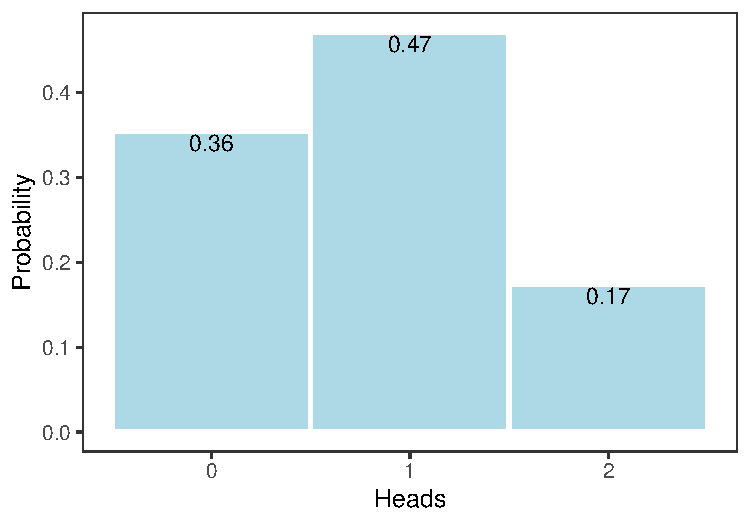
\includegraphics[width=\textwidth]{figure-latex/unnamed-chunk-7-2-1}

\end{example}

\begin{exercise}

A pair of fair 6-sided dice were rolled. Let \(X\) denote the sum of the
number of dots on the top faces.

\begin{enumerate}
\item
  Construct the probability distribution of \(X\).
\item
  Find the probability that \(X\) takes an odd value.
\end{enumerate}

\end{exercise}

\begin{exercise}

The number \(X\) of days in the summer months that a construction crew
cannot work because of the weather has the probability distribution

\begin{longtable}[]{@{}llllllllll@{}}
\toprule()
x & 6 & 7 & 8 & 9 & 10 & 11 & 12 & 13 & 14 \\
\midrule()
\endhead
P(x) & 0.03 & 0.08 & 0.15 & 0.2 & 0.19 & 0.16 & 0.1 & 0.07 & 0.02 \\
\bottomrule()
\end{longtable}

\begin{enumerate}
\item
  Find the probability that no more than ten days the construction crew cannot work in the
  summer.
\item
  Find the probability that from 8 to 12 days the construction crew cannot work in the summer.
\item
  Find the probability that no days at all the construction crew cannot work in the summer.
\end{enumerate}

\end{exercise}

\hypertarget{mean-and-standard-deviation-of-a-discrete-random-variable}{%
\subsection{Mean and Standard Deviation of a Discrete Random
Variable}\label{mean-and-standard-deviation-of-a-discrete-random-variable}}

Let \(X\) be a discrete random variable and \(p_X(x)=P(X=x)\) the
probability mass function.

\begin{itemize}
\item
  The \textbf{expected value} \(E(X)\) (also called \textbf{mean} and
  denoted by \(\mu\)) of the discrete random variable \(X\) is the
  number \[\mu=E(X)=\sum xp_X(x).\]
\item
  The \textbf{variance} \(\mathrm{Var}(X)\) (also denoted by
  \(\sigma^2\)) of the discrete random variable \(X\) is the number
  \[\sigma^2=\mathrm{Var(X)}=\sum (x-E(X))^2p_X(x).\]
\item
  The \textbf{standard deviation} \(\sigma\) of a discrete random
  variable \(X\) is the square root of its variance:
  \[\sigma=\sqrt{\sum (x-E(X))^2p_X(x)}.\]
\end{itemize}

\begin{example}

One thousand raffle tickets are sold for \$2 each. Each has an equal
chance of winning. First prize is \$500, second prize is \$300, and
third prize is \$100. Find the expected value of the net gain, and interpret
its meaning.

\end{example}

\begin{example}

The waiting time (rounded to multiples of 5) in the cafeteria at a
Community College has the following probability distribution. Find the
expected waiting time and the standard deviation.

\begin{longtable}[]{@{}llllll@{}}
\toprule()
\(x\) (minutes) & 5 & 10 & 15 & 20 & 25 \\
\midrule()
\endhead
\(P(X=x)\) & 0.13 & 0.25 & 0.31 & 0.21 & 0.1 \\
\bottomrule()
\end{longtable}

\end{example}

\begin{example}

The probability distribution of an unfair die is given in the following
table.

\begin{longtable}[]{@{}llllll@{}}
\toprule()
\(x\) & 1 & 2 & 3 & 4 & 5 \\
\midrule()
\endhead
\(P(X=x)\) & 0.18 & 0.12 & \(\,?\,\) & 0.14 & 0.23 \\
\bottomrule()
\end{longtable}

\begin{enumerate}
\item
  Find \(P(X=3)\).
\item
  Find the mean, variance and standard deviation of this probability
  distribution.
\end{enumerate}

\end{example}

\begin{exercise}

Seven thousand lottery tickets are sold for \$5 each. One ticket will
win \$2,000, two tickets will win \$750 each, and five tickets will win
\$100 each. Let \(X\) denote the net gain from the purchase of a
randomly selected ticket.

\begin{enumerate}
\item
  Construct the probability distribution of \(X\).
\item
  Compute the expected value \(E(X)\) of \(X\). Interpret its meaning.
\item
  Compute the standard deviation \(\sigma\) of \(X\).
\end{enumerate}

\end{exercise}

\hypertarget{binomial-distribution}{%
\subsection{Binomial Distribution}\label{binomial-distribution}}

\begin{itemize}
\item
  A \textbf{binomial experiment} is a probability experiment satisfying:

  \begin{enumerate}
  \item
    The experiment has a fixed number \(n\) of independent trials.
  \item
    Each trial has only two possible outcomes: a success (S) or a
    failure (F).
  \item
    The probability \(p\) of a success is the same for each trial.
  \end{enumerate}
\item
  The discrete random variable \(X\) counting the number of successes in
  the \(n\) trials is the \textbf{binomial random variable}. We say
  \(X\) has a \textbf{binomial distribution} with parameters \(n\) and
  \(p\) and write it as \(X\sim B(n, p)\).
\item
  For \(X\sim B(n, p)\), the \textbf{probability of getting exactly
  \(x\) successes in \(n\) trials} is
  \[P(X=x)=B(x,n,p)={_n C_x} p^x(1-p)^{n-x}=\frac{n!}{(n-x)!x!}p^x(1-p)^{n-x},\]
  where \(n!=n(n-1)\cdots 1\), read as \(n\) factorial, for \(n>0\) and
  \(0!=1.\)
\item
  The notation \({_n C_x}=\frac{n!}{(n-x)!x!}\) is read as \(n\) choose
  \(x\), which is the number of ways to choose \(x\) objects from a set
  of \(n\) objects.
\end{itemize}

\begin{example}

A card is randomly selected from a standard deck and replaced. This
experiment is repeated a total of \(5\) times.

\begin{itemize}
\item
  Find the probability of getting exactly \(3\) clubs.
\item
  Find the probability of getting at least \(3\) clubs.
\end{itemize}

\end{example}

\begin{exercise}

Let \(X\) be a binomial random variable with parameters \(n = 5\),
\(p=0.2\). Find the probabilities

\begin{enumerate}
\item
  \(P(X=3),\)
\item
  \(P(X<3),\)
\item
  \(P(X>3).\)
\end{enumerate}

\end{exercise}

\begin{exercise}

A manufacturing machine has a 4\% defect rate.

If 6 items are chosen at random, what is the probability that at least
one will have a defect?

\end{exercise}

\hypertarget{mean-and-standard-deviation-of-binomial-distribution}{%
\subsection{Mean and Standard Deviation of Binomial
Distribution}\label{mean-and-standard-deviation-of-binomial-distribution}}

\begin{itemize}
\item
  The mean of a binomial distribution of \(n\) trials is
  \[\mu =\sum xP(X=x)=\sum x\cdot \dfrac{n!}{(n-x)!x!}p^x(1-p)^{n-x} = np.\]
\item
  The variance of a binomial distribution of \(n\) trials is
  \[\sigma^2 =\sum (x-np)^2P(X=x)=\sum x^2P(X=x)-(np)^2=np(1-p).\]
\item
  The standard deviation of a binomial distribution of \(n\) trials is
  \[\sigma=\sqrt{np(1-p)}.\]
\item
  We consider an event \(E\) \textbf{unusual} if the probability
  \(P(E)\leq 5\%\).
\end{itemize}

\begin{example}

The probability that an egg in a retail package is cracked or broken is
0.02.

\begin{enumerate}
\item
  Find the average number of cracked or broken eggs in a one dozen
  carton.
\item
  Find the standard deviation.
\item
  Is getting at least two broken eggs unusual?
\end{enumerate}

\end{example}

\begin{exercise}

Adverse growing conditions have caused 5\% of grapefruit grown in a
certain region to be of inferior quality. Grapefruit are sold by the
dozen.

\begin{enumerate}
\item
  Find the average number of inferior quality grapefruit per box of a
  dozen.
\item
  A box that contains two or more grapefruit of inferior quality will
  cause a strong adverse customer reaction. Find the probability that a
  box of one dozen grapefruit will contain two or more grapefruit of
  inferior quality.
\end{enumerate}

\end{exercise}

\begin{exercise}

CCA has stated in 2017 that 48\% of its students are first generation
college students.

Suppose you sample 5 CCA students and ask if they are first generation
college students or not, counting the number of first generation
students.

\begin{enumerate}
\item
  Create a binomial probability distribution (table) for this situation.
\item
  Find the mean of the binomial distribution.
\item
  Find the standard deviation of this binomial distribution.
\end{enumerate}

\end{exercise}

\hypertarget{extra-practice-problems}{%
\subsection{Extra Practice Problems}\label{extra-practice-problems}}

\begin{exercise}

Find the mean and the standard deviation of the probability
distribution.

\begin{tabular}{ll}
\toprule
x & P(x) \\
\midrule
0 & 0.2 \\
1 & 0.2 \\
2 & 0.1 \\
3 & 0.5 \\
\bottomrule
\end{tabular}

\end{exercise}

\begin{exercise}

A company tracks the number of sales new employees make each day during
a 100-day probationary period. The results for one new employee are
shown at the right.

\begin{tabular}{@{}ll@{}}
  \toprule
  Sales per day \(x\) & Number of days \(f\) \\
  \midrule
  0 & 16 \\
  1 & 19 \\
  2 & 15 \\
  3 & 21 \\
  4 & 9 \\
  5 & 10 \\
  6 & 8 \\
  7 & 2 \\
  \bottomrule
  \end{tabular}

\begin{enumerate}
\item
  Find the probability of each outcome.
\item
  Construct a probability distribution table.
\item
  Find the mean of the probability distribution.
\item
  Find the variance and standard deviation.
\end{enumerate}

\end{exercise}

\begin{exercise}

A poll is given, showing 35\% are in favor of a new building project.

If 5 people are chosen at random, what is the probability that exactly 2
of them favor the new building project?

\end{exercise}
\vspace*{5\baselineskip}

\hypertarget{lab-binomial-distribution}{%
\subsection{Lab: Binomial
Distribution}\label{lab-binomial-distribution}}

Let \(X\) be a binomial random variable with parameters \(n\) and \(p\), that is \(X\sim B(n, p)\). In Excel, \(P(X=x)\) is given by\\
\texttt{BINOM.DIST(x,\ n,\ p,\ FALSE)}\\
 and \(P(X\le x)\) is given by\\
\texttt{BINOM.DIST(x,\ n,\ p,\ TRUE)}.\\
You may click input function
\(f_x\) and then search \texttt{binom} to find the function.

\begin{exercise}

A type of surgery has a 90\% chance of success. The surgery is performed
on 7 patients.

Use excel to answer the following questions.

\begin{enumerate}
\item
  Find the probability of the surgery being successful on exactly 5
  patients.
\item
  Find the probability of the surgery being successful on at least 4
  patients.
\end{enumerate}

\end{exercise}

